\section{Monitoring Approach}
\label{sec:approach}

Our monitoring approach strives to reduce the memory requirements of finite 
state monitoring. At the same time it also tries to make monitoring more 
time-deterministic without compromising much with the error reporting.
The approach is based on the following mechanisms.

\subsection{Context-based sampling}

We use context-based sampling to control the 
number of monitors. The motivation for this approach comes from our observation 
that the monitors created at the same creation site and under similar program
execution context tend to go through a similar life cycle. In other words, these monitors are more 
likely to show a redundant behavior. Hence, the heuristic applied for this 
sampling is based on the program execution context. Our approach works by i) identifying 
the monitor creation sites which are specified as creation events in the 
monitoring specification, and then by ii) obtaining the method calling sequence to identify 
the execution context, and finally by iii) making a decision about the 
allocation of the monitor based on the number of times this context was seen in 
the past. More often the monitoring system has seen the context, less likely it 
is to allocate a monitor. The program execution context that we consider in this work is
the method calling sequence of limited length. We describe the implementation details
in Section~\ref{sec:evaluation}.

\subsection{Fixed-size global pool of monitors}

We limit the total number of 
monitors that our monitoring approach would generate by creating a small 
monitor-pool of fixed size prior to the program execution and then maintaining 
it during the execution. In short our approach reuse monitors. The monitors 
after their usage can be returned back to the system. Moreover, if the pool runs 
out of monitors and the system needs a new monitor, one of the monitors currently being 
used is forcefully reclaimed and made available for the reallocation. The 
heuristic that we use to reclaim a monitor is based on the observation that the 
program events are often temporally separated. In other words, in an execution 
trace, the events related to a same receiver object are likely to be generated 
in close time intervals. We exploit this observation by making the last used potentially active 
monitor available for reallocation. This also means that the objects associated with the monitor
are not tracked further, and if any of them observe another event that might have otherwise
lead the monitor to the error state, the approach will now miss the error. 
Potentially missing a few errors is a cost of our optimized monitoring approach, 
however, by using smart heuristics presented in this Section the approach tries to
minimize \textit{false negatives}. As described in Section~\ref{sec:definition}, our
goal is to detect all nonredundant errors and not all errors.

\subsection{Fixed-size local pool of monitors for individual objects}

In the case of properties related to multiple objects, 
an object can get associated with numerous monitors in its life-time. For example,
in the case of \texttt{UnsafeIterator} property a collection object may get associated
with numerous iterator objects in its life-time. In other words, every pair of a collection and its related
iterator has an associated monitor. Hence, a collection may have several monitors associated with it
and they are stored in a map corresponding to the collection object as a key.
Therefore, an event related to the collection object results in the states of 
several monitors getting updated. Hence, handling such events may become 
\textit{nondeterministic} in terms of their execution times even when the events are related
to a same symbol, or to a same set of objects but at different times.

For this work, we consider a monitoring behaviour to be time-deterministic if we can compute the 
worst-case time taken to execute every monitoring event. Binding the number of 
monitors associated with an object allows us to limit the worst case execution 
time for any monitoring operation associated with that object. Our approach 
implements this constraint by allocating a fixed-size local pool of monitors to 
individual objects. We reallocate an existing monitor in case this buffer is full and we need a new
monitor for the same set of objects.

%Section~\ref{subsec:outline} gives the outline of our approach, and
%Section~\ref{subsec:algo} presents the algorithm.

\subsection{Outline of the approach}
\label{subsec:outline}

\begin{figure}[t]
\centering
  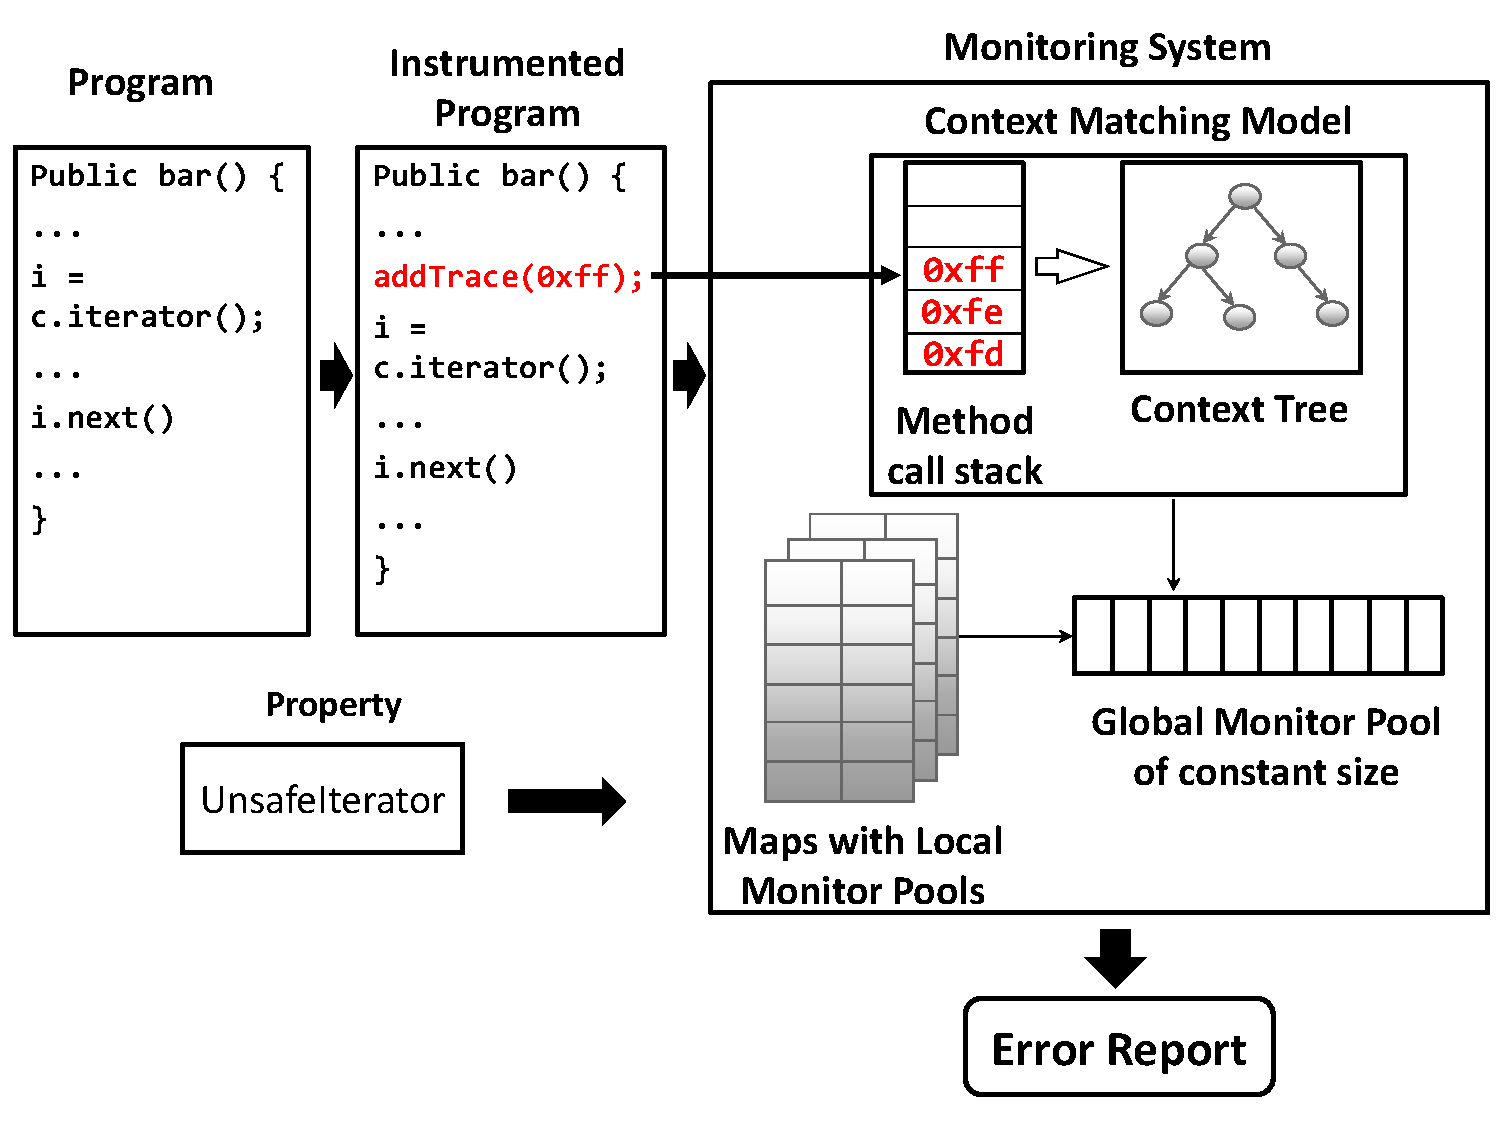
\includegraphics[scale=0.4, trim= 2cm 1cm 0 1cm]{./images/schematic.pdf}
  \caption[Schematic of Memory-efficient and Deterministic Monitoring 
System]{Schematic of Memory-efficient and Deterministic Monitoring System.}
  \label{fig:schematic}
\end{figure}

Figure~\ref{fig:schematic} shows the main elements of our approach. The program 
under execution generates events parameterized by objects which are accepted by 
our monitoring system, and each one of them is handed over to the monitor 
allocation component. This component based on the event type and the heuristics 
described in the previous sections
makes a decision about whether to allocate a monitor or not. For convenience, we 
specify the program points that generate creation events explicitly, so that the 
approach can leverage this information to make the decision about allocation. 
If the event is of creation type, the monitoring system checks the execution context and its 
tracking history to see if the context was already seen in the past, and if yes, 
then with what frequency. The system probabilistically skips the monitor 
allocation phase for frequently seen contexts. 
%The contexts are maintained as trees in which a new context adding a new branch or branches and leaf node. 
%Every leaf node uniquely defines a context and it keeps information about the 
%number of times the context was seen.
The seen contexts are stored as bitmaps to enable efficient
comparisons.

In case the system chooses to allocate a monitor, it consults the global and the 
local monitor pools to see if a fresh monitor can be allocated. I not
an old monitor is reused. This mechanism is implemented as a circular array that preserves 
the chronological ordering. In case an old monitor is chosen for tracking, that 
monitor is first removed from the existing local pools of the corresponding 
objects, and then reallocated to the new objects under consideration.

The tracking of monitors for the non-creation events is similar to the 
conventional monitoring system. The only difference is that if no monitor exists in the maps 
corresponding to objects associated with an event, then monitoring is completely 
skipped for that event. This case implies that the monitors corresponding to the 
associated objects were never created by the system, since we have distinct creation
events for properties to be monitored. Skipping monitoring events is a 
direct saving in terms of execution time overhead.




\begin{algorithm}[t]
                      % enter the algorithm environment
\caption[Algorithm]{Context-Aware Monitoring Algorithm. $\phi$ = 
($Q$,$\Sigma$,$\delta$,$q_{0}$,$F$), $\eta=(\beta, \sigma)$ where $\eta$ is an event and $\alpha \in 2^O$ 
be a set of associated objects and $\sigma \in \Sigma$}          % give the algorithm 
% a caption
\label{alg1}                           % and a label for \ref{} commands later 
% in the document
\begin{algorithmic}[1]                  
   %\STATE \textbf{let} \textit{O} be the set objects that receive events
   \STATE \textbf{let} $\Sigma_{c} \in \Sigma$ be the set of creation symbols
   \STATE \textbf{let} \textit{threshold} : $\mathcal{N} \to \mathcal{R}$ be a 
function generating a threshold value
   \STATE \textbf{let} \textit{A} be the global circular array of monitors
   \STATE \textbf{let} \textit{ObjsMons} : $O \to \textit{MS}$ be a function
   \STATE \textbf{let} \textit{MonObjs} : $M \to L$ be a function
   \STATE \textbf{let} \textit{ObjsSym} be a binary relation over L and $\Sigma$
   \STATE \textbf{let} $\pi \in \Pi$ be a finite sequence of method structures
   \STATE \textbf{let} $\zeta$ be the data structure holding the program 
execution contexts
   %\STATE \textbf{let} \textit{getFreq} : A function that takes $\psi \in \Psi$ 
% and $\eta$  and returns \textit{ct} which is the number of times the context was 
% seen
   %\STATE \textbf{let} \textit{incFreq} : A routine that takes $\psi \in \Psi$ 
% and $\eta$  and $n \in \mathcal{N}$ and sets $\psi.count$ 
   
    \IF{$\sigma \in \Sigma_{c}$}
        \STATE $\pi$  $\leftarrow$ getExecutionContextInfo()
        \IF{isMatch($\pi$, $\zeta$) = TRUE}
           \STATE $k$ $\leftarrow$ threshold($\pi$, $\zeta$)
        \ELSE
        	   \STATE $k \leftarrow 1$
        \ENDIF
        \STATE updateExecutionContext($\pi$, $\zeta$)
        \IF{Rand() $\leq k$}  
            	\STATE $m$ $\leftarrow$ $A$.nextMonitor($o$)
        		\FOR{$l' \subseteq$ MonObjs($m$)} 
            	%\IF{$\exists \sigma \in \Sigma : (l', \sigma) \in ObjsSym $}
		\STATE ObjsMons($l'$) $\leftarrow  ObjsMons(l') / \{m\}$
            	%\ENDIF   
        		\ENDFOR
        		\FOR{$l' \subseteq l $} 
            		%\IF{$\exists \sigma \in \Sigma : (l', \sigma) \in 
% ObjsSym $}
			\IF{ObjsMons($\alpha'$).size() = MAX\_MON}
				 \STATE $m' \leftarrow$ ObjsMons($\alpha'$).first();
			  	\FOR{$\alpha'' \subseteq$ MonObjs($m'$)} 
					\STATE ObjsMons($\alpha''$) $\leftarrow$  
ObjsMons($\alpha''$) / \{$m'$\}
        				\ENDFOR
			\ENDIF
                		 \STATE ObjsMons($\alpha'$) $\leftarrow$  
ObjsMons($l'$) $\cup$ \{$m$\}
            		%\ENDIF   
        		\ENDFOR
        \ENDIF
 \ENDIF
 \FOR{$m$ $\in$ ObjsMons($\beta$)}
     \STATE $m$.cur $\leftarrow$ $\delta$($m$.cur,$\sigma$)
     \IF{$m$.cur = err}
        \STATE report$\hspace{5pt}\textbf{error}$
     \ENDIF
 \ENDFOR
 
\end{algorithmic}

\end{algorithm}
\label{algo:monitoring}



\subsection{Monitoring Algorithm}
\label{subsec:algo}

Algorithm~1 depicts the steps that implement our monitoring scheme. Lines 9--32 
describe the operations that are performed when a creation event is encountered 
and a new monitor may need to be allocated. Line 10 checks the program execution 
context. If the execution context is already seen which is checked at  line 11, 
then a \textit{threshold} value is generated based on the number of times the 
context is seen in the past; else if the context is unseen, the threshold is 
assigned the highest possible value which is 1. In either case Line 16 updates 
the execution context history. In our implementation it involves either adding 
new branches in the context tree if the context was unseen or only incrementing 
the frequency count filed of the leaf node corresponding to the known context.

Lines 17--31 describe the steps when the threshold value is found to be large 
enough to justify allocation of monitor which is checked by the condition at 
line 17. As a result, a new monitor from the global circular array is allocated. 
Lines 19--21 describe the steps to reclaim the monitor in case it is previously 
assigned. This step ensures that all previous bindings are removed and the 
monitor is ready for the new assignment.

Lines 23--28 describe the steps that ensure that the local monitor pool limit is 
not reached. In case it is, the oldest monitor in the pool is reclaimed first by 
removing it from all the lists of associated object maps before the new monitor 
is added in the lists as shown by line 29.

Finally, as shown in lines 33--38, the relevant monitors are retrieved and their 
states are updated. In case any of the state is the \textit{error} state, then 
the error is reported. This final step is similar to the conventional 
monitoring, except that no monitor will be tracked if the system does not see 
any monitor allocated.


\subsubsection{Memory-Efficiency and Time-Determinism}
\label{subsubsec:efficiencyanddeterminism}

The algorithm preallocates monitors from a pool of constant size, and then if 
required, the monitors are reused. In our study we varied the pool size from 100 
to 100k monitors. This results in reducing the number of required monitors 
considerably especially for the challenging program and property combinations in 
which millions of monitors get generated. As our study indicates, our approach 
may result in a dramatic saving in the memory requirements of a software.

It is easy to see that the algorithm has worst-case time bounds for all of its 
steps making the algorithm time-deterministic. Fetching current execution 
context in the form of a call stack is an expensive but still a constant time 
operation. The execution context tree has a bounded depth which we have limited 
to three in our prototype implementation. Hence performing read or write 
operations on it as in lines 11 and 16 are time-bound operations.

Depending on the map implementations, all the map operations such as the ones on 
lines 20, 26, and 29 are constant-time operations. The \textit{for} loops on 
lines 19, 22 and 25 iterate only a small finite number of times depending on the 
number of objects involved in the event which is typically either one or two. 
The \textit{for} loop on line 33 executes at most \texttt{MAX\_MON} times since 
that is the limit on the size of local monitor pools associated with objects.

\subsubsection{Soundness, Memory, and Determinism: Tradeoffs}
\label{subsubsec:tradeoff}

There is unfortunately a tradeoff between soundness and memory and we need to 
choose one at the cost of other. However, runtime monitoring is inherently 
unsound \cite{}. It can only report what it has seen. This means program errors 
may not be reported if the paths that encounter them are not executed. We 
stretch this limitation a little bit further to achieve substantial benefits in 
terms of memory savings. Our technique should enable developers to use runtime 
monitoring in the resource-constrained system settings where the previous 
techniques for finite-state monitoring might have been seen infeasible.

Similar tradeoff exists between soundness and determinism in terms of time, but 
we believe that binding worst-case execution times has its own rewards 
especially in the domain of real-time systems. Hence, our approach tries to use 
smart heuristics based on our observations and experience so as to reduce false 
negatives and improve the soundness of the system. As indicated by the study 
presented in Section~\ref{sec:study}, our approach can save considerable amount 
memory and can also make monitoring time-determinitic. Moreover, it does not 
compromise with its \textit{completeness} by ensuring that no false positives 
are produced.

\ignore{
\section{Simple Code and Property Example:}
While JavaMOP represents state of art runtime monitoring, our goal is to limit 
the number of monitors associated with a set of objects. It typically models 
sequencing properties as finite state automata (FSA) and check whether a program 
satisfies them during runtime.  JavaMOP uses object based monitoring in which a 
monitor for a FSA property is a relation between a set of related objects 
created during program execution and a state of the FSA.  The execution of 
sequence of program statements (under test), related to both property and the 
set of related objects, corresponds to the sequence of FSA transitions.\\
\begin{figure}[h]
\centering
  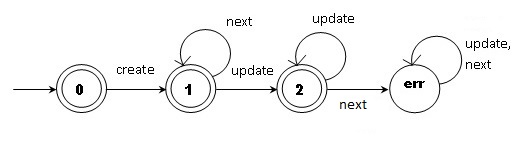
\includegraphics[scale=0.6]{./images/Unsafe.jpg}
  \caption[UnsafeIterator Property FSA]{UnSafeIterator Property.}
  \label{fig:typestateProperty FSA}
\end{figure}
\\Let us assume we are monitoring UnsafeIterator property that says not to 
modify an object of class Collection while iterating over this collection at the 
same time. In this case, it would be unclear whether the program should iterate 
over the original contents or the modified contents of the collection. While 
iterating over a collection, the runtime monitoring ensures that the program 
behaviour is well-defined. In other words, the monitor checks that there should 
not be a call to any method that is updating the collection after an iterator is 
created and before an element is accessed by a call to method next. The regular 
expression for the property is (create ; next* ; update*) and Fig 3.1 shows the 
finite state automata for UnsafeIterator property.\\\\
Below shows a code snippet for a test program. The relevant statements for the 
above property are calls to methods iterator(), add(), and next() on appropriate 
receiver objects. The relevant statements in the fragment of code being 
monitored are instrumented with extra code i.e., the OBSERVE... calls to perform 
monitoring.\\\\
When the call to method iterator() is encountered, a monitoring event create is 
generated. The instrumented code maintains a map, keyed by set of related 
objects that have been involved in previous events. The values corresponding to 
the keys are the set of monitors that are associated with the objects. On 
handling the create event, if it is found that no monitors are associated with 
the collection \textit{m1} and iterator \textit{itr}, our approach will list the 
history of method calls on the object \textit{itr} (bar(a1,a2), third(a1,a2), 
second(a1,a2), first(a1,a2), main() from our example). It will analyse if there 
exists same method calls of previously monitored objects and will sample the 
object for monitoring if match is not found and it will store the history of 
method calls for this object. However, on finding a match, the object may or may 
not be considered for monitoring depending upon how frequently it has been 
monitored previously.
\begin{center}
\textbf{A code snippet}
\begin{lstlisting}

void main(String[] args) {
	  ArrayList a1 = new ArrayList();
     al.add("C");
	  al.add("A");
	  al.add("B"); 
	  ArrayList a2 = new ArrayList ();
	  first(a1,a2);
	}
void first(ArrayList a1, ArrayList a2) { 
	  second(a1,a2); 
	} 
void second(ArrayList a1, ArrayList a2) {
	  third(a1,a2); 
	} 
void third(ArrayList a1, ArrayList a2) {
	  bar(a1,a2); 
	}
void bar(ArrayList m1,Arraylist m2) {
	  Iterator itr = m1.iterator();
		   OBSERVE.create(m1,itr);
	  m2.add(?ÄúX?Äù);
		   OBSERVE.update(m2);
     while(itr.hasNext()) {
	    Object element = itr.next();
		   OBSERVE.next(itr);
	  }
	}
    
\end{lstlisting}
\end{center}


Whenever an object is sampled for monitoring, the total number of monitors 
analysing the property are checked. If the number is below the specified limit, 
a new monitor is created and references to it are associated with the new keys 
\textit{m1} and \textit{itr} and on the other hand, if the number exceeds the 
limit, the previously generated monitor is reassigned for the current objects by 
changing the references. Thus, a limited set of monitors is used for analysing 
the property violations as done in runtime monitoring. 
}














\ignore{
\begin{algorithm}[h]
                      % enter the algorithm environment
\caption[Algorithm]{Monitoring Algorithm. $\phi$ = 
(Q,$\Sigma$,$\delta$,$q_{0}$,F), e=(l,b) where e is an event and l $\in \Sigma$ 
and b $\in O$ be the set of receiver objects}          % give the algorithm a 
caption
\label{alg1}                           % and a label for \ref{} commands later 
in the document
\begin{algorithmic}[1]                  
   %\STATE \textbf{let} \textit{O} be the set objects that receive events
   \STATE \textbf{let} $\Sigma_{c} \in \Sigma$ be the set of creation symbols
   \STATE \textbf{let} \textit{prob} determines the generation of monitor 
(Initializing it to 1).
   \STATE \textbf{let} \textit{MA} be the array of monitors
   \STATE \textbf{let} \textit{ObjMonsMap} : \textit{O} $\to$ \textit{MS} be a 
map
   \STATE \textbf{let} \textit{ObjsSym} be a binary relation over L and $\Sigma$
   \STATE \textbf{let} \textit{SE} be a finite sequence of method frames
   
    \IF{$b \in \Sigma_{c}  \lor \textit{ObjMonsMap(o)} = null$}
        \STATE $SE  \leftarrow retrieveMethodCalls(o)$
        \FOR{$SE' \subseteq SE$} 
           \STATE $match  \leftarrow
           isMatched(SE')$
        \ENDFOR
        \IF{$(match)$}
           \STATE $prob \leftarrow P(countOfMatches)$
        \ENDIF   
        \IF{$ ((\exists(rand)\subset RNG : rand < prob))$}  
            \IF{$sizeOf (MA) < limit$} 
                \STATE $ m \leftarrow new monitor(o),MA \leftarrow m $
            \ELSE
                \STATE $m \leftarrow retrieve(MA[index]) $
            \ENDIF   
            \STATE $monitoringFlag \leftarrow  true$    
        \ELSE
            \STATE $monitoringFlag \leftarrow  false$ 
        \ENDIF
        \FOR{$l' \subseteq l $} 
            \IF{$\exists \sigma \in \Sigma : (l', \sigma) \in ObjsSym $}
                \IF{$(monitoringFlag) $} 
                   \STATE $ObjsMons(l') \leftarrow  ObjsMons(l') \cup \{m\}$
                \ENDIF
            \ENDIF   
        \ENDFOR
 \ENDIF
 \FOR{$m \in MA$}
     \STATE $m.cur \leftarrow \delta(m.cur,b)$
     \IF{$(m.cur = err)$}
        \STATE report$\hspace{5pt}\textbf{error}$
     \ENDIF
 \ENDFOR
\end{algorithmic}

\end{algorithm}
}

\ignore{Runtime Monitoring is complete but fundamentally unsound since it cannot 
see anything beyond the current execution. In our approach, we sacrifice on the 
soundness to achieve memory efficiency and determinism in terms of time.	

The aim of our research is to develop optimization techniques without 
compromising heavily with the error reporting. We have developed techniques that 
identify objects in a program for which new monitors will be generated only if 
they satisfy the required probability related to the program execution context. 
We are guided by the heuristics that considers the history of method calls that 
have been invoked on the current object being monitored over the course of 
object?Äôs lifetime, from allocation to collection, as the decision factor to 
determine if the object has been previously monitored.\\\\ 
In object based monitoring, for every object that invokes a property for 
monitoring, an instance of monitor is created and all subsequent calls on those 
objects generate events[14]. It may be the case that an object A following a 
particular sequence of method calls, reaches a method where the typestate 
property of the current object is monitored for violation and there is another 
object B which follows the same method call trace as A and reaches the same 
method. Here, the conventional monitoring approach will create again a new 
monitor for the second method invocation to check for property violation 
although the objects of this method have been previously monitored. Thus, in our 
approach, we are sampling the objects that are to be monitored. The new monitor 
instances are generated for sampled objects and the objects are sampled by 
listing the history of method calls invoked on the objects.\\
Our approach is built on dynamic typestate analysis and limits the number of 
monitors that are associated with events related to a set of objects. Moreover, 
the total number of monitors generated for the typestate property checking is 
bounded explicitly in our work. A monitor pool is maintained and once the number 
of monitors generated reaches the limit specified, the already generated 
monitors are reassigned for checking the violation of the properties. This helps 
in utilizing the memory efficiently and reduces memory overhead.\\\\
For a multi-object property, those that involve more than one object such as 
\textit{UnSafeIterator} property, one \textit{Collection} object has several 
monitors associated with it at a time. This means that a single method call on 
that object can result in several monitor
update operations. The number of associated monitors can grow uncontrollably and 
it becomes difficult to keep a track of every monitor for that event, hence the 
whole operation of handling events may become non-deterministic in terms of 
execution time. By limiting the number of monitors associated, the events become 
bounded and  hence, our approach makes monitoring deterministic in terms of 
time. We provide worst-case bounds for the execution times of handling events.}
